\chapter{Ход работы}

\section{Задание на лабораторную работу}

Разработать продукционную экспертную систему на Прологе для решения
задачи по определению группы дорожного знака.

\section{Диаграммы}

\begin{figure}[H]
	\centering
	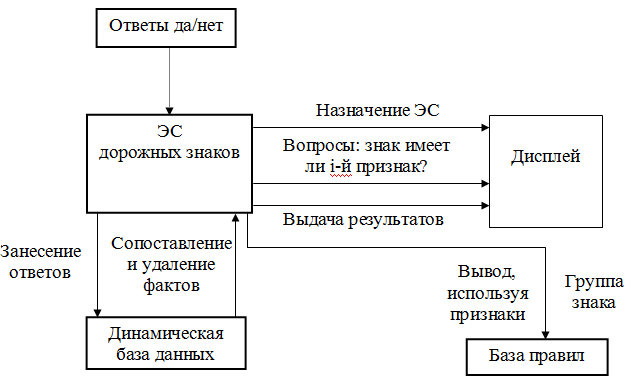
\includegraphics[width=1\linewidth]{fig/dataflow}
	\caption{Диаграмма потоков данных ЭС}
	\label{fig:dataflow}
\end{figure}

\begin{figure}[H]
	\centering
	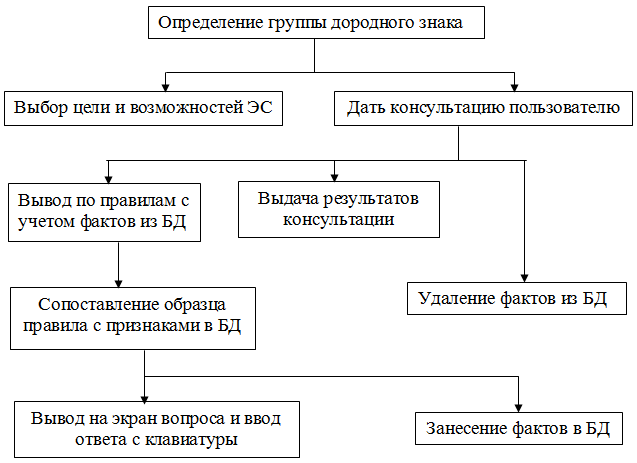
\includegraphics[width=1\linewidth]{fig/scheme}
	\caption{Структурная схема ЭС}
	\label{fig:scheme}
\end{figure}

\section{Программа на языке Prolog}

\inputminted[encoding=cp866]{prolog}{src/Prog.pro}

\begin{figure}[H]
	\centering
	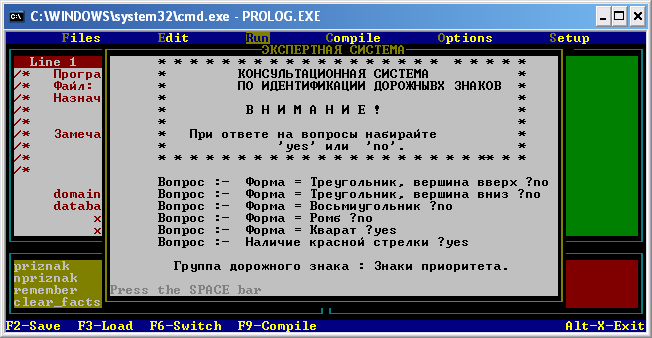
\includegraphics{fig/screen1}
	\caption{Тестирование продукционного правила 6}
	\label{fig:screen1}
\end{figure}

\begin{figure}[H]
	\centering
	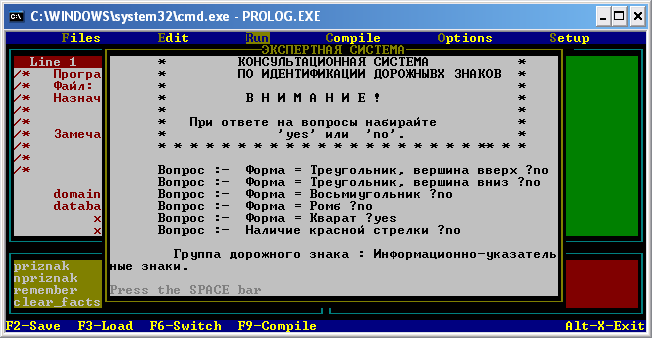
\includegraphics{fig/screen2}
	\caption{Тестирование продукционного правила 5}
	\label{fig:screen2}
\end{figure}

\begin{figure}[H]
	\centering
	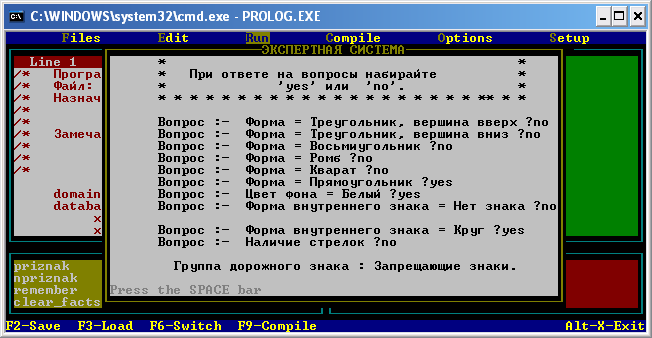
\includegraphics{fig/screen3}
	\caption{Тестирование продукционного правила 15}
	\label{fig:screen3}
\end{figure}

\begin{figure}[H]
	\centering
	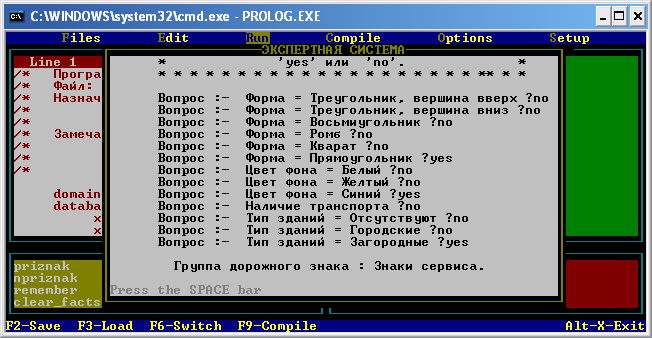
\includegraphics{fig/screen4}
	\caption{Тестирование продукционного правила 21}
	\label{fig:screen4}
\end{figure}
